\section{Case Study: Arbitrary Code Execution in \textit{Super Mario World}}

One great example of arbitrary code execution not being used for evil can be found in speedruns and tool-assisted play of various classic video games. In essence, a speedrun is trying to beat a video game as quickly as possible; using glitches and other unintended tricks are generally allowed and encouraged.

In several classic video games (such as \textit{Super Mario World} for the SNES), glitches exist that allow arbitrary code execution to be possible. The methods for performing and taking advantages of these glitches varies from game to game, but they tend to exist more often in older video games due to the smaller memory capacities of the retro consoles and the somewhat questionable techniques game developers used to overcome the constraints. Most cases of arbitrary code execution in video games simply result in jumping to a certain instruction in game code (e.g. the final credits) to skip large portions of the game. However, some games can be coerced into a state where inputs from the controller directly map to assembly instructions being executed by the console. This is known as total control.

To showcase an example of how powerful arbitrary code execution can be for speedruns, we will examine the methods used to beat \textit{Super Mario World} in under two minutes by a human player \cite{dotsarecool_2015}.

\subsection{Constructing the Arbitrary Code}

The basis of this glitch is that the player is able to use an array in the game's memory that normally stores the positions of various sprites on screen as a set of instructions to be executed that will ultimately jump game execution to the final credits. This array that stores sprite locations has a maximum size of 12 elements, and whenever a new sprite is rendered on screen, it tries to place it in the highest available index in the array. Because of this, the lower elements in the array are only ever accessed or changed when there is a large number of sprites on the screen, which makes it easy to keep them at the values the player wants. In the pursuit of efficiency, sprite positions are only ever updated when the sprite moves, and are not cleared when a sprite leaves the screen for any reason. This means sprites can be placed in a very specific location, despawned using in-game mechanics, then as long as a new sprite is not ever placed in that sprite slot, the memory still has the correct values.

Conveniently, at the very beginning of the first level, a large number of enemies appear on screen and fill up the entire sprite array (this was probably placed there by the game designers to showcase how many enemies the game can handle at once on the new hardware the game was released on). The player can very carefully despawn these enemies (by eating them and spitting them out with Yoshi) at very specific locations to write some machine code to be executed later.

\begin{figure}
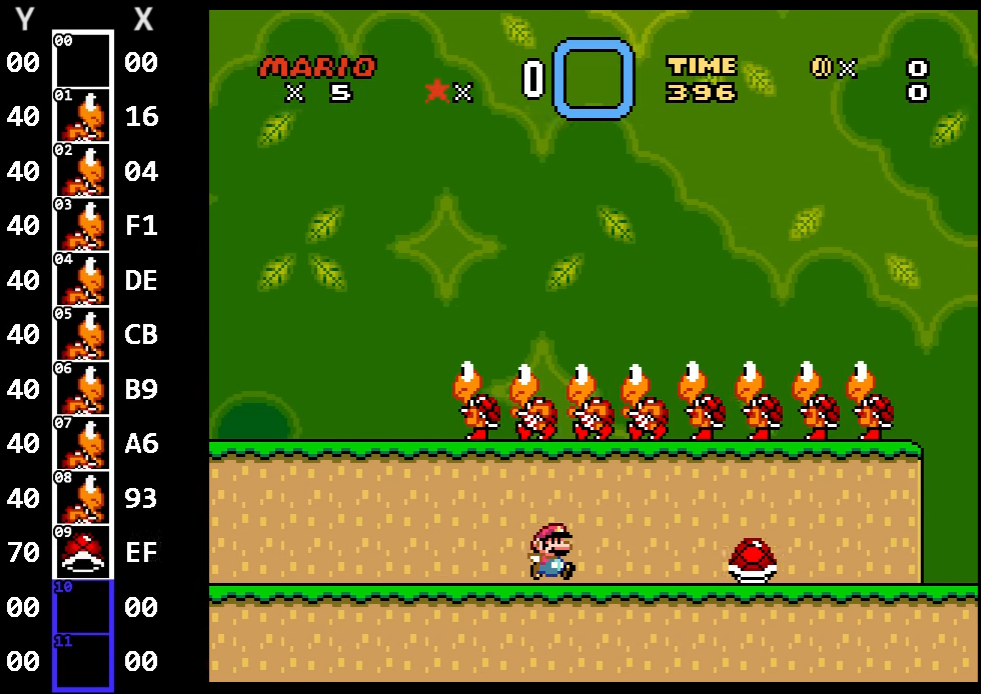
\includegraphics[width=\linewidth]{smw1.png}
\caption{The large number of enemies at the beginning of the game. To the left is a visualization of the sprite array, showing the low-bytes of Y and X positions of each sprite. These values are what is turned into code to be executed later on. \cite{dotsarecool_2015}}
\end{figure}

Once the code has been written using sprites, the player can then execute a very complicated glitch that allows program execution to jump to the sprite array's location in memory. The glitch involves attempting to eat a normal item with Yoshi at a specific spot in the level at the exact same time Mario jumps off of Yoshi and moves the screen to the right. When the screen moves enough to the right, it spawns another enemy in the level. However, since the item being eaten has already been despawned, the enemy spawns in the same sprite slot it was just occupying. Since Yoshi is still in the process of eating whatever item was in that sprite slot, it is able to eat the enemy that is not normally able to be eaten.

\subsection{Executing the "Shell" Code}

\begin{figure}
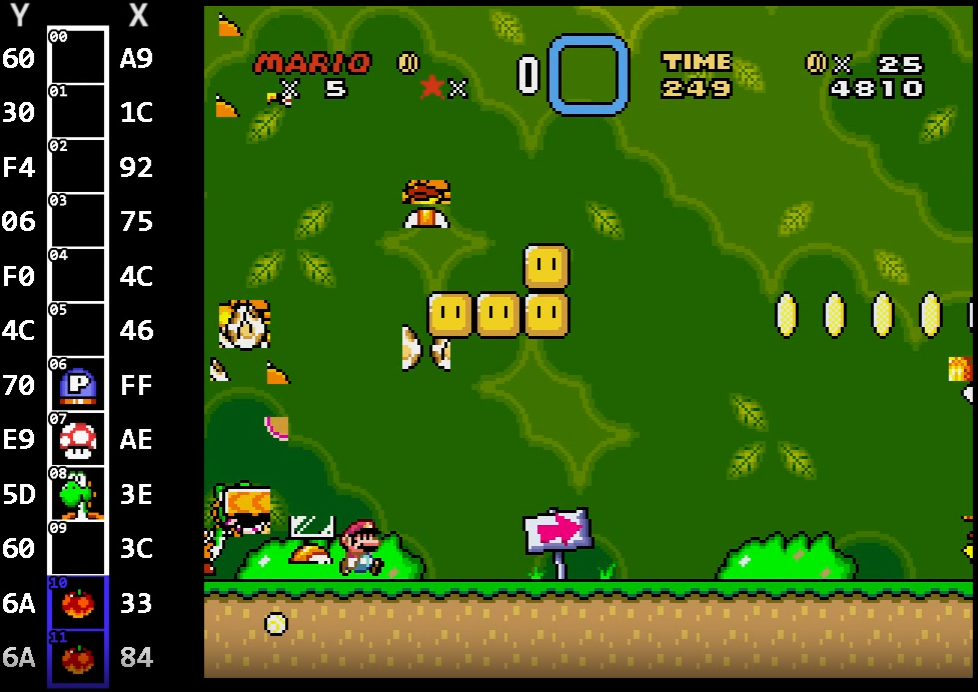
\includegraphics[width=\linewidth]{smw2.png}
\caption{The graphical glitches that occur when jumping to the boss-drawing subroutine. On the left, the same sprite array visualization shows the now complete machine code written via the X-positions of the first 7 sprite slots. \cite{dotsarecool_2015}}
\end{figure}

When Yoshi eats objects in \textit{Super Mario World}, the game looks at a large array of memory locations mapped to each eatable object (this is called a jump table). However, since the enemy being eaten isn't supposed to be in this array in the first place, the index the game tries to access in the jump table is way out of bounds and the game attempts to jump execution to an essentially random place in memory. This location isn't actually random, but it's the result of turning some other memory in the game near the jump table into an address and jumping to it. The other memory it reads happens to be the Y-position of the last particle objects drawn on the screen, which the player was also able to manipulate.

\subsubsection{Machine Code Explanation}

After performing this jump instruction from eating the invalid memory, the game is able to work its way into the sprite array and start executing code from there. The code written in the sprite array is the following:

      \begin{lstlisting}
      LDA #$1C   // A9 1C
      STA ($75)  // 92 75
      JMP $FF46  // 4C 46 FF
      \end{lstlisting}

\texttt{LDA \#\$1C}: Load the value \texttt{1C} into the accumulator. \texttt{1C} corresponds to the game mode that tells the game to fade out and start playing the credits.

\texttt{STA (\$75)}: Store the accumulator value indirectly at the address \texttt{\$75}. The address \texttt{\$75} is \texttt{01} if Mario is swimming, and \texttt{00} otherwise. Address \texttt{\$76} is \texttt{01} if Mario is facing right and \texttt{00} if Mario is facing left. As long as Mario is facing right and not swimming at the time the glitch is performed, the value \texttt{1C} will be stored at address \texttt{01 00}, which is where the current game mode is stored in memory.

\texttt{JMP \$FF46}: Normally, eating an invalid enemy would crash the game, so execution is jumped to a subroutine intended to draw a specific boss on the screen. This subroutine causes some interesting graphical glitches, but doesn't crash the game. Once the subroutine returns, the game realizes its state is the credits and launches the proper routine to to start playing them, thus beating \textit{Super Mario World}.
